\xchapter{Método de pesquisa}
{Este capítulo apresenta a metodologia utilizada para coleta e análise dos
dados do ecossistema de software acadêmico de análise estática}
\label{metodologia}

%Discutir o uso do tipo "documental", mais usado em ciências sociais e humanas. 
% document analysis conducted as a content analysis
%Foi feita uma revisão da literatura, de artigos em bases de dados -- não se pode perder isso de vista.
%Tenho visto o termo "estudo retrospectivo" sendo usado para se referir ao passado.
%estudo do tipo documental, descritivo-exploratório e retrospectivo?

%Este trabalho apresenta uma pesquisa exploratória, do tipo documental, com o
%objetivo principal de aprimorar o conhecimento a respeito da sustentabilidade
%do ecossistema de software acadêmico de análise estática.

%Hipótese geral: O ecossistema de software acadêmico de análise
%estática sofre sérios problemas de sustentabilidade, causando retrabalho,
%impedindo a colaboração e desacelerando o avanço geral do campo de pesquisa de
%análise estática.

%Lembrar de destacar o contexto (ASE, SCAM, etc.)
Este trabalho apresenta um estudo de caso exploratório ({\it exploratory case
study}) \cite{stol2015holistic} sobre a sustentabilidade do ecossistema de
software acadêmico de análise estática.
% exploratória ou descritiva? exploratória

% Decidir se será HIPOTESE geral ou QUESTAO DE PESQUISA principal.
Hipótese geral: o atual modelo de desenvolvimento de software do ecossistema de
software acadêmico de análise estática é insustentável.

% Q1: O ecossistema de software acadêmico de análise estática sofre %sérios problemas de sustentabilidade?
% Q2: Quais os tipos de problema?
% Q3: ...

% compartilhamento é um requisito para colaboração
% disponibilidade é um requisito para colaboração
% licenças expressas previamente são requisitos para colaboração
% visibilidade do software é requisito para colaboração
% preocupação com sustentabilidade e qualidade dos produtos é requisito para colaboração

%, uma suíte de ferramentas
%para análise de código fonte.

%O Analizo, apesar de ter sido utilizado especialmente para coleta de dados,
%será apresentado em detalhes no Capítulo \ref{analizo} pois ele faz parte
%também do contexto e motivação deste trabalho.

\section{Definição}

% Por que o estudo será realizado?

O que sabemos sobre a sustentabilidade técnica de projetos de software acadêmico publicados em conferências
de Engenharia de Software? Como estes projetos são mencionados na literatura acadêmica?   
Colocar QUESTAO SOBRE COLABORACAO.

\subsection{Definição do Objetivo}

\begin{description}
\item{\bf Objeto de estudo.} 
O objeto de estudo são projetos de software acadêmico de análise estática e sua sustentabilidade técnica.

\item{\bf Propósito.} 
O propósito deste estudo é caracterizar a sustentabilidade técnica de cada software acadêmico de análise estática,
trazendo informações que permitam ...

\item{\bf Perspectiva.} 
A perspectiva considerada é a de cientistas e pesquisadores, isto é, 
o cientista ou pesquisador gostaria de conhecer ecossistemas de software acadêmico de análise estática
em termos de sua sustentabilidade técnica. 
Além disso, pessoas da indústria podem estar interessadas em conhecer
software acadêmico de análise estática para financiá-lo.

\item{\bf Foco de qualidade.} 
O principal aspecto de qualidade estudado é a sustentabilidade sócio-técnica,
com destaque para três aspectos: transparência, complexidade e adoção.
%, A, B, C ... EXPLICAR A, B, C.


Q1 é demográfica?
Transparência: aberto? disponível? transparente?  Funciona? Ver Q2.
Adoção: ver Q4.
Q3? Parece que há duas questões em uma. Você vai olhar todas as versões para tratar da visibilidade??
A outra questão tem a ver sobre como referenciar software em artigos científicos?
Complexidade: qualidade do código.  Estudo 2.

\item{\bf Contexto.} 
O estudo foi conduzido com projetos de software acadêmico de análise estática
publicados nas conferências ASE e SCAM.
\end{description}

\subsection{Sumário da Definição}

%% QUERO DISCUTIR SE SUSTENTABILIDADE JA EH MENCIONADA OU NAO no Object of Study

%% GQM template

Analisar a \textit{software acadêmico de análise estática e sua sustentabilidade técnica} % object of study
com o propósito de \textit{caracterizar}  % purpose  % era medir e avaliar - coloquei 'caracterizar' 
com respeito a \textit{disponibilidade de código, números de citações e complexidade estrutural (manutenibilidade)}  % quality focus
na perspectiva do \textit{pesquisador} e do \textit{cientista}% perspective
no contexto de \textit{software acadêmico de análise estática publicado nas conferências ASE e SCAM 
e referenciado por artigos publicados nas bases da ACM e IEEE}. % context
%


\subsection{Questões de Pesquisa}

Neste estudo as seguintes questões de pesquisa, a respeito do ecossistema de
software acadêmico de análise estática, serão investigadas:

\newcommand{\QuestaoUm}{Como as taxas de publicação contribuindo com novos projetos de software acadêmico nas conferências ASE e SCAM mudam ao longo do tempo?}
\newcommand{\QuestaoDois}{Os projetos estão disponíveis para obtenção hoje? Os projetos incentivam ativamente a contribuição? Os espaços do projeto são abertos e transparentes?}
\newcommand{\QuestaoTres}{Como a visibilidade dos artefatos de software publicados nas conferências ASE e SCAM mudam ao longo do tempo? Como os artefatos de software acadêmico publicados nas conferências ASE e SCAM são mencionados na literatura acadêmica ao longo do tempo?}
\newcommand{\QuestaoQuatro}{Como as taxas de entrada de novos atores cientistas usuários finais de software acadêmico mudam ao longo do tempo? Os projetos possuem contribuidores além dos autores iniciais?}

\begin{description}
  \item [Q1:] \QuestaoUm
  \item [Q2:] \QuestaoDois
  \item [Q3:] \QuestaoTres
  \item [Q4:] \QuestaoQuatro
\end{description}

%\subsection{Resultados}

%\begin{enumerate}
%  \item Caracterização do ecossistema de software acadêmico de análise estática
%  \item Reflexão sobre os problemas de sustentabilidade sofridos pelo ecossistema de software acadêmico de análise estática
%  \item Formulação de hipóteses sobre os problemas de sustentabilidade sofridos pelo ecossistema de software acadêmico de análise estática
%\end{enumerate}

\subsection{Métricas}

Para responder às questões de pesquisas, as seguintes métricas serão usadas:
\begin{enumerate}
\item métricas relacionadas ao ecossistema do software (número
total de lançamentos, data e número de versão de cada lançamento, número de
commits, número de contribuidores); % estudo3
\item métricas relacionadas à qualidade interna do software (complexidade estrutural do código fonte). % estudo3
\item métricas de publicação (número de citações, número de menções, número de usos).) %estudo2
\end{enumerate}

%\section{Planejamento do Estudo} \label{sec:study1:planning}

% Como o estudo será conduzido?

%%%%%%%%%%%%%%%%%%%%%%%%%%%%%%%%%%%%%%%%%%%%%%%%%%%

%No segundo estudo, os softwares com código fonte disponível foram avaliados em
%relação a sua manutenabilidade através da métrica de complexidade estrutural. A
%coleta dessa métrica para cada software foi realizada pelo Analizo, uma suíte
%de ferramentas para análise de código fonte, e está sendo considerado como um
%indicador de manutenabilidade.

%Um conjunto de softwares de análise estática da indústria foi incluído nesta
%etapa, todos os dados coletados para os softwares acadêmicos foram também
%coletados para este novo conjunto. Esses softwares foram então caracterizados em
%relação à frequencia de lançamentos, linguagem de programação e o tipo de
%entrada suportado.

%Questão de pesquisa:

%* Como ocorre o co-desenvolvimento dos softwares
%* Como acontece colaboração na construção dos softwares
%* Como os softwares contribuem para a construcao de conhecimento novo em novas pesquisas derivadas

% * mais da metade desenvolvem seus próprios softwares
% * falta de visibilidade gera questionamentos sobre qualidade
% * falta de treinamento leva a produzir softwares sem qualidade
% * produtividade científica requer capacidade de replicação
% * capacidade de replicação depende de qualidade

%(mover os coding schema para anexos ou (nao) e manter todos os campos incluindo os de howison
%e os meus, em cada etapa vou preenchendo mais dados, na seleção estruturada pego o mínimo,
%na próxima coleta preencho com mais questões, criador, etc)

%será
%aplicado automaticamente com auxílio de um script desenvolvido durante este
%trabalho de pesquisa, detalhes deste script, outros artefatos produzidos
%durante esta pesquisa, e onde obtê-los pode ser encontrado no Apêndice
%\ref{reproducibilidade-do-estudo}.

%\begin{verbatim}
%  "tool" OU "framework"; E
%  "download" OU "available"; E
%  "http" OU "ftp"; E
%  "static analysis" OU "parser".
%\end{verbatim}

%As informações coletadas sobre cada software inclui nome, descrição e o
%endereço onde obter uma cópia, normalmente página web ou repositório de código
%fonte, esses endereços foram verificados para confirmar se os softwares estão,
%de fato, disponíveis.

%segundo as definições de software {\it
%livre} e {\it open} da Free Software
%Foundation\footnote{\url{https://www.gnu.org/philosophy/free-sw.html}} e Open
%Source Initiative\footnote{\url{https://opensource.org/osd}}, respectivamente,

%#### artigos nao encontrados para download:
%
%  url = {http://doi.acm.org/10.1145/3090064.3090070},

% * revisão estruturada
%    paper{step} = 'structured-review';
% * citações ao software
%    citations{key}{step} = 'review-citations';

% contribuições sem peso:
% =======================
% o software mudou de nome, qual o nome antigo, qual o novo nome
% um novo software foi criado a partir daqui, qual o nome do novo
% um novo software foi criado com base neste

%O antipositivismo, por outro lado, postula que toda a verdade é construída
%socialmente, o que significa que os seres humanos criam sua própria verdade
%sobre as questões de relevância para elas e essas verdades socialmente
%construídas são válidas e valiosas.

%as próprias pessoas, introduzem aspectos que são especialmente difíceis de capturar.
%Entretando, estudos tentando capturar comportamento
%humano como isto se relaciona ao engenharia de software tem aumentado e, não
%surpreendentemente, estão aumentando o uso empregando de métodos qualitativos

%O pesquisador positivista vê a verdade objetiva quanto possível, ou seja,
%existe alguma verdade absoluta sobre as questões de relevância, mesmo que essa
%verdade seja evasiva e que o papel da pesquisa seja cada vez mais próximo
%disso.

%O estudo de engenharia de software tem sido complexo e difícil. A complexidade
%surge de questões técnicas, do desastrada intersecção entre máquina as
%capacidades (ou qualidades?) humanas e de máquina, e do papel central que
%pessoas tem na realização de tarefas da engenharia de software.

%Os primeitos dois aspectos oferecem mais do que apenas problemas complexos para
%manter os pesquisadores de engenharia de software empírica ocupados. Mas o
%último fator, as próprias pessoas, introduzem aspectos que são especial,ente
%difíceis de capturar. Entretando, estudos tentando capturar comportamento
%humano como isto se relaciona ao engenharia de software tem aumentado e, não
%surpreendentemente, estão aumentando o uso empregando de métodos qualitativos

%Veja Creswell (1998) para uma explicação
%mais completa do positivismo, do interpretivismo, de outros quadros filosóficos
%relacionados e do papel dos métodos de pesquisa qualitativa neles.
%   weightless\_contributions={},

%Os métodos qualitativos são apropriados para (mesmo, implicitamente) pesquisa
%positivista em engenharia de software, e um pesquisador não precisa se
%inscrever de todo o coração para a visão de mundo interpretativa
%(antipositivista) para aplicá-los.

%Os dados qualitativos são dados representados como texto e imagens, não números (Gilgun, 1992).

%O foco deste capítulo é bastante estreito, na medida em que se concentra em
%apenas algumas técnicas, e apenas alguns dos possíveis projetos de pesquisa que estão bem
%adequado para tópicos comuns de pesquisa em engenharia de software. Veja Judd et al. (1991),
%Lincoln e Guba (1985), Miles e Huberman (1994) e Taylor e Bogdan
%(1984) para descrições de outros métodos qualitativos.

%A apresentação deste capítulo divide métodos qualitativos para aqueles para
%coletando dados e aqueles para análise de dados. Exemplos de vários métodos são fornecidos
%para cada um, e os métodos podem ser combinados entre si, bem como com
%métodos quantitativos.

%Ao longo deste capítulo, serão extraídos exemplos de
%vários estudos de engenharia de software, incluindo (von Mayrhauser e Vans 1996;
%Guindon et al., 1987; Lethbridge et al., 2005; Perry et al. 1994; Lutters and Seaman,
%2007; Singer, 1998; Orlikowski 1993).

%Exemplos mais detalhados também serão usados
%de estudos descritos em Parra et al. (1997) e Seaman e Basili (1998) porque
%eles representam a experiência do autor (tanto positiva como negativa).

%A Computação muitas vezes é vista como uma disciplina de
%engenharia. Existe a engenharia de software, a engenharia de
%computação e a engenharia de computadores, cada qual com
%um objetivo diferenciado, mas sendo que todas têm em
%comum a produção de conhecimento para aplicação em
%processos de produção de software, sistemas ou hardware.

%A ciência aplicada muitas vezes é confundida com a
%tecnologia. Mas, como será visto adiante, são coisas distintas.

%A perspectiva crítica entende o mundo como a construção histórica e social
%de relações de poder e dominação. Nesta visão sistemas de informação pro-
%vavelmente herdam da sociedade relações de poder, alienação e dominação,
%e revelar essas heranças é o objetivo central da pesquisa qualitativa de fundo
%crítico. [Myers and Young. 1997] é um bom exemplo de pesquisa qualitativa de
%fundo crítico em CC.

%Para muitos pesquisadores de ciências sociais, os métodos qualitativos são
%reservados exclusivamente para uso de pesquisadores antipositivistas e não devem
%ser misturados com métodos quantitativos ou pontos de vista positivistas.

%Os métodos de pesquisa qualitativa foram projetados,
%principalmente por pesquisadores educacionais e outros cientistas sociais
%(Taylor e Bogdan, 1984), para estudar as complexidades de humanos (por exemplo,
%motivação, comunicação, compreensão).


%Numa primeira definição, métodos qualitativos diferem de métodos quanti-
%tativos porque se ocupam de variáveis que não podem ser medidas, apenas
%observadas. Essa é uma dicotomia muito simplista. Métodos qualitativos vêm
%das ciências sociais, em oposição aos métodos quantitativos que derivam das
%ciências naturais.

%Essa diferença na origem já é suficiente para que visões
%diferentes sobre o que é ciência, e como se faz ciência, tornem definições sus-
%cintas sobre o que é um ou outro método muito difícil.


%surgiram de um 
%Historicamente, os métodos de pesquisa qualitativos surgiram da tradição
%interpretativa, ou antipositivista, na pesquisa em ciências sociais.
%O antipositivismo, por sua vez, surgiu como uma reação ao positivismo, que foi
%e continua a ser o fundamento filosófico prevalecente (implícito) da pesquisa
%em ciências naturais e físicas, incluindo a ciência da computação e a
%engenharia de software.

%se presta a combinar recursos qualitativos e métodos quantitativos, a fim de
%aproveitar os pontos fortes de ambos.

%pelo encontro de qualidades
%humanas e de máquinas, e o papel central que as pessoas desempenham nas tarefas
%da engenharia de software. Os aspectos humanos são especialmente difíceis de
%capturar e tem chamado atenção e atraído métodos de pesquisa e coletada de
%dados tradicionais de outros campos, especialmente, das ciências sociais.
%
%ciencias formais: logica e matematica, na computação: teoria dos algoritmos, linguagens formais, autômatos
%ciencias empiricas:
%  ciencias naturais: astronomia, fisica, quimica, na computação: eletronica, circuito logicos
%  ciencias sociais: historia, psicologia, sociologia, na computação: informatica na educação, comércio eletrônico, games, IHC
%
%ciencias puras: formal (lógica) ou empírica (cosmologia), na computação: pouca atuação e presença da computação ainda
%ciencias aplicadas: engenharias, na computação: engenharia de software, informatica na educação, etc
%
%ciencias exatas: matemática, física, química, na computação: a computação é uma ciência exata, a princípio
%ciencias inexatas: metereologia, economia, maioria ciencias sociais, na computação: algoritmos geneticos, casos de redes neurais
%
%ciencias duras: rigor cientifico em observações, experimentos, etc
%  ciencias duras formais: muito uso de logica e matematica
%  ciencias duras naturais: costumam depender de estatistica, exige rigor na comprovação de resultados empiricos, medicina
%
%ciencias moles: aceitam evidencias via estudos de caso por exemplo
%
%ciencias duras X ciencias moles, computação: normalmente entende-se computação como ciência dura, mas ainda
%                                             existe dificuldade de providenciar dados ....
%
%


%Contrário a fontes como [Myers 1997], que classifica a pesquisa qualitativa
%em 4 grupos, eu acho a divisão em apenas dois grupos mais produtiva: a
%pesquisa observacional e a pesquisa-ação (action research).

%A pesquisa
%observacional tem como objetivo observar o ambiente, mas não modificá-lo; já
%o objetivo central da pesquisa-ação é modificar o ambiente.

%É claro que só a
%presença do pesquisador causa alguma modificação no ambiente, mas essa
%modificação não é o objetivo da pesquisa observacional, e algumas variantes
%da pesquisa observacional tentam eliminar esse efeito.

%Segundo vários autores (por exemplo [Orlikowski and Baroudi 1991]) a pes-
%quisa qualitativa onservacional pode ser dividida segundo a perspectiva filosó-
%fica ou epistemológica que a embasa em:
%
%positivista
%interpretativista
%crítica
%
%Eles também são usados para responder o "porquê" às perguntas já
%abordadas pela pesquisa quantitativa.

%Normalmente entende-se a Computação como uma ciência
%dura, mas a realidade ainda, em muitos casos é que os
%pesquisadores têm dificuldade em providenciar dados em
%quantidade suficiente para dar suporte empírico a suas
%conclusões. Assim é que se vêem ainda muitos artigos em
%Computação que utilizam um ou alguns poucos estudos de
%caso para tentar “validar” uma técnica, modelo ou teoria.
%Como visto adiante, o estudo de caso é uma excelente fonte de
%dados para uma pesquisa exploratória, mas, a não ser no caso
%de contradição de uma teoria comumente aceita, o estudo de
%caso não valida a hipótese em estudo.

%Embora a posição filosófica implícita predominante dessas áreas
%de pesquisa permaneça positivista.
%Historicamente os métodos de pesquisa da ciência
%da computação e engenharia de software se fundamentam em filosofias opostas
%ao que fizeram surgir os métodos qualitativos, assim como as ciências naturais
%e físicas.

%Os métodos são descritos aqui em termos de como eles poderiam ser usados em um estudo que
%mistura métodos qualitativos e quantitativos, como muitas vezes são em estudos de software
%Engenharia.

%Eles ajudam a responder perguntas que envolvem variáveis difíceis
%de quantificar (particularmente a característica humana como
%motivação, percepção e experiência).

%outros campos, especialmente, das ciências sociais.
%Métodos qualitativos, então, foram necessários para capturar e descrever essas
%realidades socialmente construídas.

%Há desvantagens no
%entanto.  A análise qualitativa é geralmente mais intensiva em mão-de-obra em
%comparação com análise quantitativa. Os resultados qualitativos geralmente são
%considerados "mais suaves/leves" ou "Mais confusos/fuzzier" do que resultados
%quantitativos, especialmente em comunidades técnicas como a nossa.  Eles são
%também mais difíceis de resumir ou simplificar.

%A principal vantagem da pesquisa bibliográfica reside no fato de permitir ao
%investigador a cobertura de uma gama de fenômenos muito mais ampla do que
%aquela que poderia pesquisar diretamente

%A pesquisa bibliográfica também é indispensável nos estudos históricos

%Enquanto a pesquisa bibliográfica se utiliza fundamentalmente das contribuições
%dos diversos autores sobre determinado assunto, a pesquis"ã documental yale-se
%de materiais que não recebem ainda um tratamento analítico, ou que ainda podem
%ser reelaborados de acordo com os objetos da pesquisa

%A pesquisa bibliográfica é desenvolvida com base em material já elaborado,
%constituído principalmente de livros e artigos científicos

%Uma vantagem da pesquisa documental é que os documentos constituem fonte rica e
%estável de dados

%Outra vantagem da pesquisa documental está em seu custo

%Outra vantagem da pesquisa documental é não exigir contato com os sujeitos da
%pesquisa

%\cite{wazlawick2015metodologia}

%por exemplo, em pesquisadores em sistemas de
%informação, interação homem-computador e engenharia de software.
%emprestado a experiência acumulada dos cientistas sociais aplicadas no contexto
%da computação, 

%De um modo geral, métodos qualitativos em ciência da computaçao são métodos que
%se caracterizam por ser um estudo aprofundado de um sistema no ambiente onde
%ele está sendo usado, ou, em alguns casos, onde se espera que o sistema seja
%usado. Métodos qualitativos sempre envolvem pessoas, e na maioria das vezes
%sistemas.

%A metodologia adotada neste estudo para a coleta de dados é do tipo: A técnica
%de coleta de dados utilizada neste trabalho é a Consulta Documental a materiais
%escritos de diferentes tipos dos registros ....  ; manuais, relatórios e outros

%3.3. Independent Techniques
%       3.3.1. Analysis of Electronic Databases of Work Performed
%       3.3.2. Analysis of Tool Logs
%       3.3.3. Documentation Analysis
%       3.3.4. Static and Dynamic Analysis of a System
%4.2. Coding and Analyzing the Data
%\cite{singer2008software}

%Estudos em engenharia de software descrevemos uma série de técnicas de coleta
%de dados para esses estudos, organizados em torno de uma taxonomia com base no
%grau em que a interação com engenheiros de software é necessária.

%mas pouco se sabe sobre como os engenheiros de software realizam seu
%trabalho. Para melhorar as ferramentas e a prática de engenharia de software,

%A principal vantagem de usar métodos qualitativos é que eles forçam a
%pesquisador para investigar a complexidade do problema em vez de abstrai-lo.
%Assim, os resultados são mais ricos e mais informativos. Técnicas
%independentes, ou seja, são técnicas caracterizadas pela ausencia da
%necessidade de interação entre pesquisador e com os atores sendo estudados.

%, sendo marcada por
%aspectos comportamentais humanos, 
%bastante

%essencialmente por
%questões humanas e de máquinas, e o papel que as pessoas desempenham nas
%tarefas da prática em engenharia de software, os aspectos humanos são
%especialmente difíceis de capturar e tem atraído a atenção dos cientistas para
%métodos de pesquisa pouco usuais, tanto em estudos da ciência da computação,
%quanto da engenharia de software.

%se presta a
%combinar métodos qualitativos e quantitativos, a fim de aproveitar os pontos
%fortes de ambos. A pesquisa de engenharia de software tem sido bastante
%atrasada para reconhecer o valor dos estudos qualitativos. Esta atenção tem
%sido notada nas últimas décadas, por exemplo, através da adoção de métodos
%qualitativos, especialmente em estudos de campo voltados para estudar
%profissionais reais à medida que resolver problemas reais.

%estudo de campo, com coleta de dados através de pesquisa documental

%\cite{brooks2008replication}
%\cite{wainer2007metodos}
%\cite{singer2008software}
%\cite{wazlawick2015metodologia}

%A engenharia de software, apesar de ser uma atividade marcada fortemente por
%aspectos técnicos e humanos, tem sido lenta em reconhecer o valor do método de
%pesquisa qualitativo e seu alto potencial para investigar a complexidade de
%problemas reais sem necessidade de abstrai-los, fonecendo resultados ricos e
%informativos, especialmente sobre questões relacionadas a crenças,
%experiências, atitudes e opiniões de indivíduos ou grupos
%\cite{seaman1999qualitative}.

%, com as seguintes características
%principais:

%estratégia de pesquisa: trabalho de campo
%método de pesquisa: exploratory case study,

%Adotamos uma estratégia de pesquisa de trabalho de campo (Field Studies),
%segundo o framework apresentado em \citeonline{stol2015holistic}, de
%configuração natural (Natural Settings),

%modelo de ciclo de vida, staged, simples, chris comentou, tem modelo adaptado pra SL
%lançou pro mundo, começa a evoluir, rtem vida, depois de muito tempo começa a decair, para de
%evoluir e passa a ser serviço, com poucas coisas novas, tem gente 
%
%pessoal da espanha daptou esse modelo para o SL rajlich
%
%A staged model for the software life cycle
%VT Rajlich, KH Bennett - Computer, 2000 - ieeexplore.ieee.org
%
%Adapting the staged model for software evolution to free/libre/open source software
%A Capiluppi, JM González-Barahona, I Herraiz… - … Principles of software …, 2007 - dl.acm.org

%novos conhecimentos e uma compreensão mais profunda dos fenômenos investigados
%* without any intervention by the researchers.
%* focuses on a particular phenomenon, organization or system
%* level of generalizability to a large population is much lower (due to the specific context)
%* to study software professionals or software systems
%* do not include any deliberate modification of the environment in which the research is conducted
%* having a low level of precision of measurement or control as would be found in laboratory experiments
% \item conduzida numa configuração de mundo real
% \item máximo no realismo do contexto
%Maximizes realism of context
%Low on precision of measurement
%Low on generalizability of results

%\begin{itemize}
%  \item Com o foco num fenômeno, organização ou sistema em particupar
%  \item Com um baixo nível de generalização e alto realismo do contexto
%  \item Sem intervenção do pesquisador no ambiente
%\end{itemize}

%STRATEGIES:
%
% * I    Field Studies +‘maximum’ in realism of context
% * I    Field Experiments
%
% * II   Experimental Simulations
% * II   Laboratory Experiments
%
% * III  Judgment Tasks
% * III  Sample Surveys
%
% * IV   Formal Theory
% * IV   Computer Simulations

%duas dimensões principais: obtrusiveness e generality
%                           ‘intrusion’

%As configurações em que as estratégias de pesquisa são adotadas variam,
%four different types of research settings; I, II, III, IV

%I     Natural Settings
%      * the researcher has no goal to make any changes or control any variables of interest
%      * intrusao em Field Experiments é maior que em Field Studies

%II    Contrived Settings
%      * artificially created by a researcher for the sole purpose of the study
%      * top of the ‘obtrusiveness’, maior controle que Field Experiment, Laboratory Experiments tem o maximo de controle

%III   Setting-Independent
%      * aim to gather observations of behavior (people, systems) that is independent from the setting
%      * Judgment Tasks are used to elicit responses from a set experts, or judges about a certain topic
%      * Sample Surveys aim to gather data from a larger group of respondents and as such usually have a better generalizability

%IV    No Empirical Setting
%      * are not empirical strategies but rather are theoretical.

%The choice of research strategy, ‘big picture’

%(( Runkel and McGrath derived a framework to position different research strategies [29] \cite{runkel1972research} ))

%A ``estratégia de pesquisa'' tem um impacto significativo sobre o que pode e
%não pode ser alcançado em um estudo em termos de aquisição de novos
%conhecimentos e uma compreensão mais profunda dos fenômenos investigados
%\cite{stol2015holistic}.

%Utilizamos como estratégia de 
%\cite{seaman1999qualitative}.

%Exemplos de
%seus resultados são o código-fonte, a documentação e os relatórios. Os
%subprodutos são criados no processo de trabalho, por exemplo, solicitações de
%trabalho, trocas de logs e saída do gerenciamento de configuração e ferramentas
%de compilação. Esses repositórios ou arquivos podem servir como fonte primária
%de informações.

%Este trabalho apresenta uma pesquisa exploratória, do tipo documental, com o
%objetivo principal de aprimorar o conhecimento a respeito da sustentabilidade
%do ecossistema de software acadêmico de análise estática.

% Third degree: Independent analysis of work artifacts where already available and sometimes compiled data is used. This is for example the case when documents such as requirements specifications and failure reports from an organization are analyzed or when data from organizational databases such as time accounting is analyzed.


\section{Analizo}

Analizo \cite{Terceiro2010Analizo} é um conjunto de ferramentas para análise de código-fonte e
visualização com suporte a múltiplas linguagens de programação, software livre,
extensível e capaz de lidar com código-fonte não mais compilável. A capacidade
de lidar com código-fonte não mais compilável permite analisar código-fonte
com erros de sintaxe, com referências a bibliotecas não mais disponíveis, ou
que usem bibliotecas com mudanças de API.

%Ela será a ferramenta utilizada por nós durante este estudo para análise do
%código-fonte das ferramentas selecionadas, a decisão pela ferramenta Analizo
%se deu por conta dela ser também a escolha utilizada nos trabalhos
%relacionados (seção \ref{trabalhos-relacionados}) onde estamos nos apoiando,
%além disso, Analizo também tem sido utilizada em diversos estudos
%desenvolvidos em nosso grupo de pesquisa (seção \ref{trabalhos-analizo}).

%% \section{Arquitetura do Analizo}
%%
%% A arquitetura do Analizo é apresentada na Figura \ref{arquitetura-analizo}
%% através de uma representação {\it Layered Style} \cite{Clements2002}, cada
%% camada no diagrama usa apenas os serviços oferecidos pela camada diretamente
%% abaixo dela.
%%
%% \begin{figure}[h]
%% \center
%% 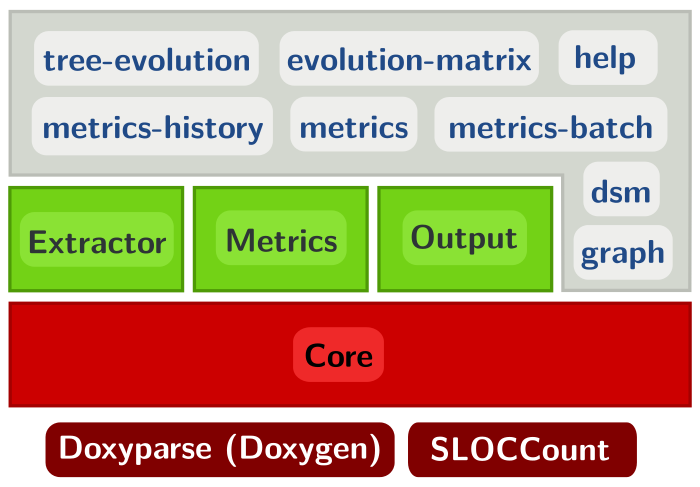
\includegraphics[scale=0.3]{imagens/analizo-architecture.png}
%% \caption{Arquitetura do Analizo, usando Layered Style \cite{Clements2002}}
%% \label{arquitetura-analizo}
%% \end{figure}
%%
%% O {\it Core} contém as estruturas de dados usadas para armazenar informações a
%% respeito do código-fonte sendo analisado, lista de módulos\footnote{o
%% conceito ``módulo'' é usado como um termo abrangente para designar diferentes
%% tipos de estruturas usados em desenvolvimento de software, como classes e
%% arquivos fonte C}, elementos dentro de cada módulo (atributos, variáveis,
%% métodos, funções) e informações de dependência (chamada, herança, etc). Esta
%% camada implementa a maior parte da lógica de negócio do Analizo, e não depende
%% de nenhuma outra camada.
%%
%% A camada {\it Extractor} lida com as informaçoes de código-fonte obtidas pelas
%% diferentes estratégias implementadas no Analizo. Os extratores obtém
%% informações do código-fonte e armazenam em estruturas de dados na camada {\it
%% Core}. Adicionar um novo extrator requer apenas a criação de uma nova subclasse
%% que faça interface com uma ferramenta externa ou que ela própria realize análise
%% de código-fonte.
%%
%% Atualmente existem dois extratores, ambos fazem interface
%% com ferramentas externas de análise estática de código-fonte:
%%
%% \begin{itemize}
%%
%%   \item {\it Analizo::Extractor::Doxyparse} é uma interface para o Doxyparse,
%%   um parser de código-fonte para C, C++ e Java desenvolvida por nosso grupo de
%%   pesquisa\cite{Costa2009}. Doxyparse é baseado no
%%   Doxygen\footnote{doxygen.org}, um sistema de documentação multi-linguagem.
%%
%%   \item {\it Analizo::Extractor::Sloccount} é uma interface para o
%%   Sloccount\footnote{dwheeler.com/sloccount} desenvolvido por David A. Wheeler,
%%   uma ferramenta que calcula o número efetivo de linhas de código.
%%
%% \end{itemize}
%% A camada {\it Metrics} processa as estruturas de dados do {\it Core} para
%% calcular métricas, até o momento Analizo suporta um conjunto razoável de
%% métricas (listadas na Seção \ref{metricas}), uma representação desta camada
%% pode ser vista no diagrama da Figura \ref{arquitetura-metrics-analizo}.
%%
%% A camada {\it Output} é responsável por lidar com diferentes formatos de
%% arquivos.  Atualmente, apenas o formato DOT é implementado no Analizo para
%% representar grafo de dependencia, adicionar novos formatos é simplesmente
%% adicionar novas classes nesta camada.
%%
%% \begin{figure}[h]
%% \center
%% 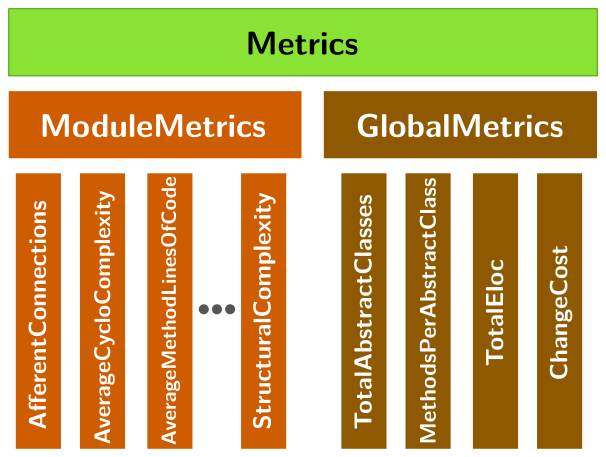
\includegraphics[scale=0.4]{imagens/analizo-metrics-architecture.png}
%% \caption{Arquitetura do módulo metrics em detalhes, usando Layered Style \cite{Clements2002}}
%% \label{arquitetura-metrics-analizo}
%% \end{figure}
%%
%% A última camada, {\it Tools}, fornece um conjunto de ferramentas de linha de comando que
%% constituem a interface do analizo, tanto para usuários finais quanto para
%% aplicações de mais alto nível. Estas ferramentas usam serviços providos pelas
%% outras camadas: eles instanciam as estruturas de dados do {\it Core},
%% inicializam um ou mais extratores, opcionalmente executam o processador de
%% métricas, instanciam um módulo de formato de saída, e gerencia todos eles para
%% prover o resultado desejado. A maioria das funcionalidades descritas na Seção
%% \ref{funcionalidades} são implementadas nesta camada.
%%
%% Estas ferramentas são pensadas na filosofia UNIX: fazem uma tarefa
%% especializada e geram uma saída que pode ser utilizada como entrada para outras
%% ferramentas, seja para o próprio Analizo ou para ferramentas externas. Algumas
%% das ferramentas implementadas no Analizo são feitas consumindo saída gerada por
%% outra ferramenta, outras são desenhadas para prover saída em formato específico
%% para aplicações externas, por exemplo, programas para desenho de grafos ou
%% visualização de dados.

\subsection{Funcionalidades}\label{funcionalidades}

\begin{itemize}

\item {\bf Análise de código-fonte multi-linguagem}

Atualmente Analizo suporta análise de código-fonte escrito em C, C++ e Java.
Entretanto, pode ser facilmente estendido para suportar outras linguagens pois
pode potencialmente suportar as inúmeras outras linguagens suportadas pelo Doxygen.

\item {\bf Métricas}\label{metricas}

O Analizo suporta tanto métricas em nível de projeto, que é calculada para todo o projeto,
quanto métricas em nível de módulos, que é calculado individualmente para cada módulo.
No nível de projeto, Analizo também provê estatística descritiva básica para cada métrica em
nível de módulo: soma, média, mediana, moda, desvio padrão, variância, skewness e kurtosis da
distribuição, valores mínimo e maximo. As seguintes métricas são suportadas até o momento:

\begin{itemize}

  \item Métricas em nível de projeto: Change Cost, Total Abstract Classes,
  Total Coupling Factor, Total Effective Lines of Code, Total Lines of Code,
  Methods per Abstract Class, Total Number of Modules, Total number of modules
  with at least one defined attributes, Total number of modules with at least
  one defined method, Total Number of Methods.

  \item Métricas em nível de módulo: Afferent Connections per Class, Average
  Cyclomatic Complexity per Method, Average Method Lines of Code, Argument with
  'nonnull' attribute passed null, Average Number of Parameters per Method,
  Allocator sizeof operand mismatch, Assigned value is garbage or undefined,
  Bad deallocator, Bad free, Coupling Between Objects, Dead assignment,
  Divisions by zero, Double free, Depth of Inheritance Tree, Dereference of
 null pointer, Dereference of undefined pointer value, Potential buffer
  overflow in call to 'gets', Lack of Cohesion of Methods, Lines of Code,
  Memory leak, Max Method LOC, Number of Attributes, Number of Children, Number
  of Methods, Number of Public Attributes, Number of Public Methods,
  Out-of-bound array access, Offset free, Potential insecure temporary file in
  call 'mktemp', Response for a Class, Result of operation is garbage or
  undefined, Return of stack variable address, Stack address stored into global
  variable, Structural Complexity, Undefined allocation of 0 bytes,
  Use-after-free, Uninitialized argument value.

\end{itemize}

É possível especificar que certos diretórios dentro do projeto não devem ser
analisados, de forma que o Analizo ignore tais arquivos durante a análise e o
cálculo de métricas.

%\item {\bf Processamento em lote}\label{lote}
%
%A maioria dos estudos quantitativos em engenharia de software envolve aquisição
%de métricas de código-fonte de um grande número de projetos, processar cada
%projeto individualmente é pouco prático, passível de erros e difícil de
%repetir. Analizo pode processar multiplos projetos em lote e produzir arquivo
%de dados CSV com métricas de cada projeto, bem como um resumo com as métricas
%em nível de projeto de todos os projetos. Estes arquivos de dados podem ser
%facilmente importados em ferramentas de estatística ou planilhas para análise
%futura. Esta capacidade de processar em lote pode também ser utilizada para
%analisar várias versões de um mesmo projeto, especialmente útil em estudos
%sobre evolução de software.


%% Este processamento em lote pode se beneficiar de processamento paralelo dando
%% mais agilidade e na análise e reduzindo o tempo total de processamento.  A
%% saída pode ser também escrita diretamente em um banco de dados relacional ao
%% invés de gerar arquivos CSV. Outro recurso voltado à performance é um sistema
%% de cache para as informações previamente calculadas, evitando repetição de
%% processamento.

%\item {\bf Histórico de métricas}
%
%Algumas vezes pesquisadores precisam processar o histórico de projetos de
%software de uma forma mais escalável. Analizo pode processar repositórios de
%controle de versão e prover arquivo de dados CSV com valores de métricas para
%cada revisão onde o código-fonte foi alterado no projeto, ou pode também gravar
%os valores diretamente num banco de dados ao invés de usar arquivos CSV. Repositórios Git e
%Subversion são suportados diretamente, repositórios CVS devem ser convertidos
%para Git de forma manual.

%\item {\bf Grafo de dependência}
%
%Analizo pode gerar saída com informações sobre dependência entre as entidades
%do projeto em um formato adequado para processamento por ferramentas de
%renderização de grafos do Graphviz\footnote{graphviz.org}. A Figura
%\ref{sample-graph} apresenta um exemplo de grafo desenhado pela ferramenta {\it
%dot} do Graphviz a partir da saída gerada pelo Analizo {\it graph}.
%
%\begin{figure}[h]
%\center
%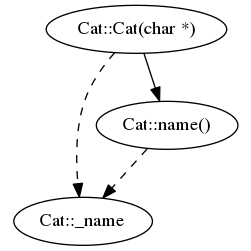
\includegraphics[scale=0.4]{imagens/sample-graph.png}
%\caption{Exemplo de grafo de dependência}
%\label{sample-graph}
%\end{figure}

%% \item {\bf Matriz de evolução}
%%
%% Outra funcionalidade útil do Analizo é a visualização de matrizes de evolução
%% \cite{Lanza2001}. Ao processar cada release de um projeto (ver Seção
%% \ref{lote}), o usuário pode solicitar a criação de uma matriz de evolução a
%% partir de arquivos de dados individuais. A Figura \ref{sample-evolution-matrix}
%% apresenta um exemplo de uma matriz produzida pelo Analizo.
%%
%% \begin{figure}[h]
%% \center
%% 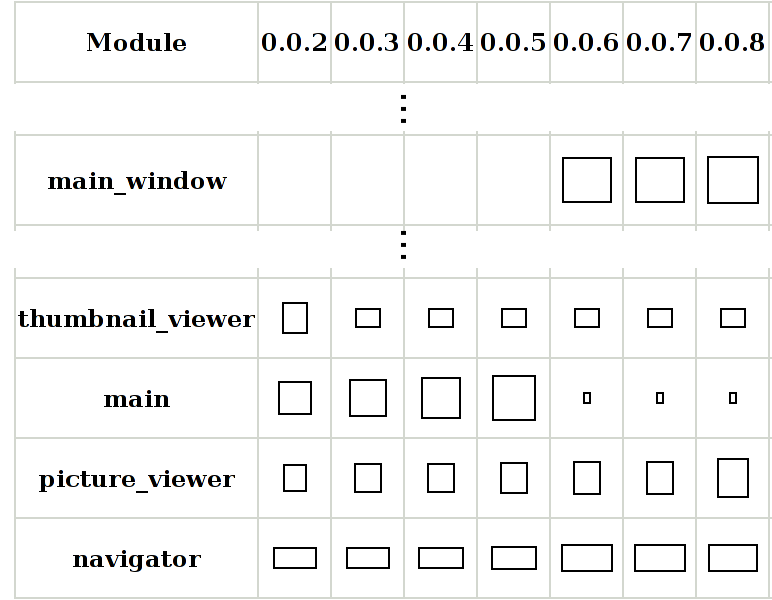
\includegraphics[scale=0.2]{imagens/sample-evolution-matrix.png}
%% \caption{Exemplo de matriz de evolução}
%% \label{sample-evolution-matrix}
%% \end{figure}
%%
%% \item {\bf Matriz de estrutura de projeto}
%%
%% Uma funcionalidade recente do Analizo é a representação visual do
%% relacionamento entre os módulos do projeto em forma de uma matriz de estrutura
%% de projeto ({\it Design Structure Matrix}) \cite{Maccormack2006}, uma DSM é a
%% representação de um grafo de dependência em forma de uma matriz quadrada. Um
%% exemplo gerado pelo Analizo pode ser visto na Figura \ref{sample-dsm}.
%%
%% \begin{figure}[h]
%% \center
%% 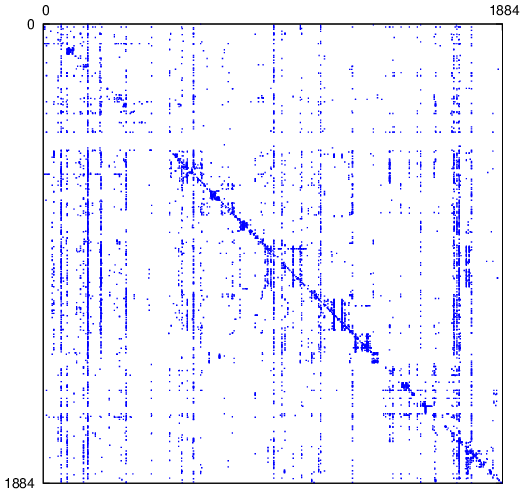
\includegraphics[scale=0.3]{imagens/sample-dsm.png}
%% \caption{Exemplo de matriz de estrutura de projeto}
%% \label{sample-dsm}
%% \end{figure}

\end{itemize}

